\documentclass[10pt,a4paper,landscape]{article}
\usepackage[T1]{fontenc}
\usepackage[utf8]{inputenc}
\usepackage{lmodern}
\usepackage[margin=12mm]{geometry}
\usepackage[table]{xcolor}
\usepackage{tikz}
\usetikzlibrary{arrows.meta,positioning,shapes.geometric,fit,calc}
\usepackage[most]{tcolorbox}
\usepackage{tabularx}
\usepackage{array}
\usepackage{enumitem}
\usepackage{fancyhdr}
\usepackage{hyperref}
\usepackage{listings}
\usepackage{draftwatermark}
\usepackage{amssymb}

\definecolor{Navy}{HTML}{10253F}
\definecolor{Blue}{HTML}{2563EB}
\definecolor{Teal}{HTML}{0F8F83}
\definecolor{Green}{HTML}{16803A}
\definecolor{Amber}{HTML}{C26A0A}
\definecolor{Red}{HTML}{B42318}
\definecolor{Ink}{HTML}{172033}
\definecolor{Muted}{HTML}{526071}
\definecolor{Line}{HTML}{D7DEE8}
\definecolor{PaleBlue}{HTML}{EEF4FF}
\definecolor{PaleTeal}{HTML}{EAF8F6}
\definecolor{PaleGreen}{HTML}{ECF8EF}
\definecolor{PaleAmber}{HTML}{FFF5E8}
\definecolor{PaleRed}{HTML}{FDECEC}
\definecolor{Paper}{HTML}{F8FAFC}

\renewcommand{\familydefault}{\sfdefault}
\setlength{\parindent}{0pt}
\setlength{\parskip}{4pt}
\setlist[itemize]{leftmargin=5mm,itemsep=1.5mm,topsep=1mm}
\hypersetup{colorlinks=true,urlcolor=Blue,linkcolor=Blue,pdftitle={Jev vs LLM: Safe Refund Workflow},pdfauthor={Netsetos}}

\SetWatermarkText{\sffamily\bfseries NETSETOS}
\SetWatermarkScale{2.15}
\SetWatermarkAngle{32}
\SetWatermarkColor[gray]{0.93}

\pagestyle{fancy}
\fancyhf{}
\fancyfoot[L]{\scriptsize\color{Muted}NETSETOS | Student Handout}
\fancyfoot[C]{\scriptsize\color{Muted}Jev vs LLM: Safe Refund Workflow}
\fancyfoot[R]{\scriptsize\color{Muted}\thepage}
\renewcommand{\headrulewidth}{0pt}
\renewcommand{\footrulewidth}{0.3pt}

\tcbset{
  clean/.style={enhanced,boxrule=0pt,arc=3mm,left=5mm,right=5mm,top=4mm,bottom=4mm},
  border/.style={enhanced,boxrule=0.7pt,arc=3mm,left=4mm,right=4mm,top=3mm,bottom=3mm,colframe=Line}
}

\newcommand{\pageheading}[2]{%
  {\Large\bfseries\color{Navy}#1}\hfill{\small\bfseries\color{Teal}#2}\par
  \vspace{1mm}{\color{Line}\rule{\textwidth}{0.7pt}}\vspace{3mm}
}
\newcommand{\pill}[2]{\tcbox[on line,boxrule=0pt,arc=3mm,colback=#1,left=2.5mm,right=2.5mm,top=1mm,bottom=1mm]{\scriptsize\bfseries\color{Ink}#2}}

\tikzset{
  flow/.style={rounded corners=3mm,draw=Line,line width=0.7pt,minimum height=20mm,text width=34mm,align=center,inner sep=3mm,font=\small},
  compact/.style={rounded corners=2.5mm,draw=Line,line width=0.7pt,minimum height=17mm,text width=27mm,align=center,inner sep=2mm,font=\scriptsize},
  arrow/.style={-{Latex[length=3mm,width=2mm]},line width=1.1pt,draw=Navy},
  reviewarrow/.style={-{Latex[length=3mm,width=2mm]},line width=1pt,draw=Red,dashed}
}

\lstdefinestyle{netsetos}{
  basicstyle=\ttfamily\scriptsize,
  backgroundcolor=\color{Paper},
  frame=single,
  rulecolor=\color{Line},
  frameround=tttt,
  breaklines=true,
  showstringspaces=false,
  columns=fullflexible,
  xleftmargin=2mm,
  xrightmargin=2mm,
  aboveskip=1mm,
  belowskip=1mm
}

\begin{document}

% PAGE 1
\begin{tcolorbox}[clean,colback=Navy,coltext=white]
  {\Huge\bfseries Jev vs LLM}\par
  \vspace{1mm}{\Large Designing a safe refund workflow}\par
  \vspace{2mm}{\small A focused student reference based on the video scenario}
\end{tcolorbox}

\vspace{3mm}
\begin{minipage}[t]{0.58\textwidth}
  \begin{tcolorbox}[border,colback=PaleAmber]
    {\large\bfseries Scenario}\par
    \vspace{1mm}
    A customer writes: \textbf{``You charged me twice. Refund the extra payment.''}
    \vspace{2mm}

    The message tells us what the customer \textbf{claims}. It does not prove that two settled charges exist, that the second charge is refundable, or that a refund has not already been issued.
  \end{tcolorbox}

  \vspace{3mm}
  \begin{tcolorbox}[clean,colback=PaleRed]
    \centering
    {\LARGE\bfseries\color{Red} CLAIM $\neq$ VERIFIED FACT}
  \end{tcolorbox}

  \vspace{3mm}
  {\small\color{Muted}\textbf{Core rule:} Model output can describe, classify, score, or route a request. Money movement must be controlled by verified records and deterministic policy.}
\end{minipage}\hfill
\begin{minipage}[t]{0.39\textwidth}
  \begin{tcolorbox}[border,colback=PaleTeal]
    {\large\bfseries\color{Teal} Safe architecture in one line}\par
    \vspace{3mm}
    \centering
    \pill{PaleTeal}{JEV ROUTES}\\[3mm]
    $\downarrow$\\[2mm]
    \pill{PaleGreen}{CODE VERIFIES + ACTS}\\[3mm]
    $\downarrow$\\[2mm]
    \pill{PaleBlue}{LLM EXPLAINS}
  \end{tcolorbox}

  \vspace{3mm}
  \begin{tcolorbox}[border,colback=white]
    {\bfseries Student objective}\par
    Know exactly where probabilistic prediction stops and application authority begins.
  \end{tcolorbox}
\end{minipage}

\vfill
\begin{minipage}[t]{0.32\textwidth}
\begin{tcolorbox}[border,colback=PaleTeal]
\textbf{Jev owns}\par
Focused decisions such as department, urgency, and refund intent, returned as constrained values with probabilities.
\end{tcolorbox}
\end{minipage}\hfill
\begin{minipage}[t]{0.32\textwidth}
\begin{tcolorbox}[border,colback=PaleGreen]
\textbf{Backend owns}\par
Identity checks, transaction lookup, policy evaluation, idempotency, authorization, execution, and audit logs.
\end{tcolorbox}
\end{minipage}\hfill
\begin{minipage}[t]{0.32\textwidth}
\begin{tcolorbox}[border,colback=PaleBlue]
\textbf{LLM owns}\par
A clear customer explanation based only on the confirmed status, amount, timing, and refund reference.
\end{tcolorbox}
\end{minipage}

\newpage

% PAGE 2
\pageheading{End-to-end architecture}{FROM CLAIM TO CONFIRMED OUTCOME}

\begin{center}
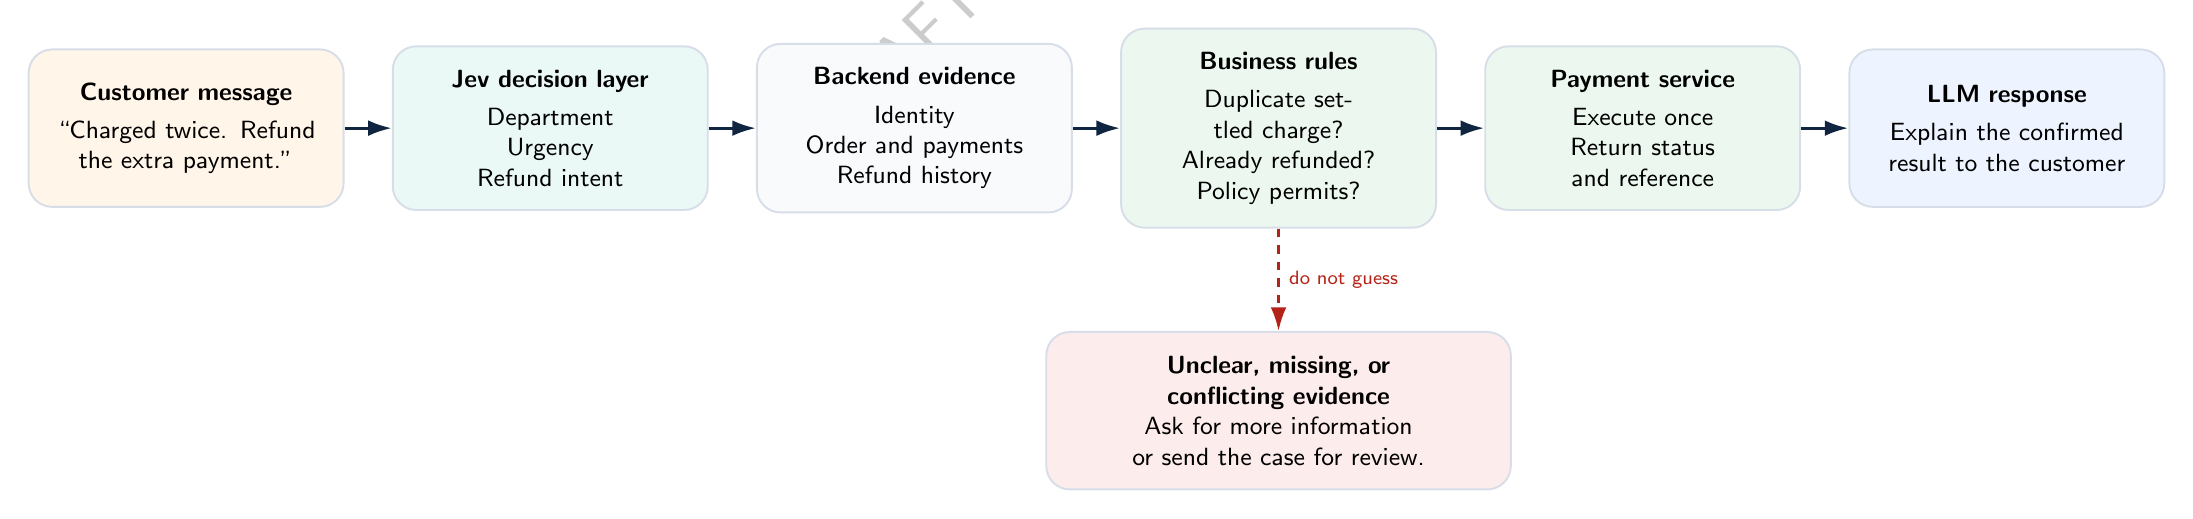
\begin{tikzpicture}[node distance=6mm]
  \node[flow,fill=PaleAmber] (message) {\textbf{Customer message}\\[1mm]``Charged twice. Refund the extra payment.''};
  \node[flow,fill=PaleTeal,right=of message] (jev) {\textbf{Jev decision layer}\\[1mm]Department\\Urgency\\Refund intent};
  \node[flow,fill=Paper,right=of jev] (records) {\textbf{Backend evidence}\\[1mm]Identity\\Order and payments\\Refund history};
  \node[flow,fill=PaleGreen,right=of records] (rules) {\textbf{Business rules}\\[1mm]Duplicate settled charge?\\Already refunded?\\Policy permits?};
  \node[flow,fill=PaleGreen,right=of rules] (payment) {\textbf{Payment service}\\[1mm]Execute once\\Return status and reference};
  \node[flow,fill=PaleBlue,right=of payment] (llm) {\textbf{LLM response}\\[1mm]Explain the confirmed result to the customer};

  \draw[arrow] (message) -- (jev);
  \draw[arrow] (jev) -- (records);
  \draw[arrow] (records) -- (rules);
  \draw[arrow] (rules) -- (payment);
  \draw[arrow] (payment) -- (llm);

  \node[flow,fill=PaleRed,text width=53mm,below=13mm of rules] (review) {\textbf{Unclear, missing, or conflicting evidence}\\Ask for more information or send the case for review.};
  \draw[reviewarrow] (rules.south) -- node[right,font=\scriptsize\color{Red}]{do not guess} (review.north);
\end{tikzpicture}
\end{center}

\vspace{5mm}
\begin{tcolorbox}[border,colback=white]
\centering
{\large\bfseries\color{Navy}
MESSAGE $\rightarrow$ JEV $\rightarrow$ DEPARTMENT $\cdot$ URGENCY $\cdot$ INTENT}
\par\vspace{3mm}
{\large\bfseries\color{Navy}
IDENTITY $\rightarrow$ ORDER $\rightarrow$ DUPLICATE CHARGE $\rightarrow$ REFUND HISTORY}
\par\vspace{3mm}
{\large\bfseries\color{Navy}
PAYMENT CONFIRMS $\rightarrow$ STATUS + REFERENCE $\rightarrow$ LLM EXPLANATION}
\end{tcolorbox}

\vspace{4mm}
\begin{minipage}[t]{0.49\textwidth}
\begin{tcolorbox}[border,colback=PaleTeal]
\textbf{What Jev contributes}\par
It turns shared text or structured state into typed, focused judgments with probabilities. That output can help software choose a route or decide when to escalate.
\end{tcolorbox}
\end{minipage}\hfill
\begin{minipage}[t]{0.49\textwidth}
\begin{tcolorbox}[border,colback=PaleGreen]
\textbf{What actually authorizes the refund}\par
Verified payment records plus deterministic business rules. The model does not hold the payment credentials or bypass policy checks.
\end{tcolorbox}
\end{minipage}

\newpage

% PAGE 3
\pageheading{Jev and a generative LLM}{BOTH CAN CLASSIFY, BUT THEIR ROLES DIFFER}

\begin{minipage}[t]{0.48\textwidth}
\begin{tcolorbox}[border,colback=PaleBlue]
{\Large\bfseries\color{Blue} Typical generative LLM}\par
\vspace{5mm}
\centering
{\LARGE\bfseries TOKEN $\rightarrow$ TOKEN $\rightarrow$ TOKEN}
\par\vspace{5mm}
\raggedright
A generative LLM normally produces text autoregressively. It can also be constrained to JSON, but the application still needs schema validation and must prevent generated language from becoming authorization.
\end{tcolorbox}
\end{minipage}\hfill
\begin{minipage}[t]{0.48\textwidth}
\begin{tcolorbox}[border,colback=PaleTeal]
{\Large\bfseries\color{Teal} Jev focused decisions}\par
\vspace{5mm}
\centering
{\LARGE\bfseries Q1 $\parallel$ Q2 $\parallel$ Q3}
\par\vspace{5mm}
\raggedright
TypeSafe describes Jev as evaluating declared questions against the same state and returning constrained answers plus probabilities. Independent questions can be evaluated together.
\end{tcolorbox}
\end{minipage}

\vspace{5mm}
\rowcolors{2}{Paper}{white}
\begin{tabularx}{\textwidth}{>{\bfseries\color{Navy}}p{37mm} X X}
\rowcolor{Navy}
\color{white}Dimension & \color{white}\textbf{Generative LLM} & \color{white}\textbf{Jev / System One model}\\
Primary output & Generated text or structured text & Typed choices, scores, and boolean-style probabilities\\
Useful here for & Explaining a confirmed outcome in natural language & Classifying, routing, scoring, and identifying intent\\
Execution pattern & Output tokens are normally generated sequentially & Declared independent questions are evaluated together\\
Critical boundary & JSON does not itself authorize a refund & Probability does not prove transaction evidence\\
Selection rule & Measure quality, latency, cost, reliability, and operational fit & Measure the same factors on the same production-like test set\\
\end{tabularx}

\vspace{5mm}
\begin{tcolorbox}[clean,colback=PaleAmber]
\textbf{Benchmarking note.} TypeSafe publishes substantial speed and cost claims for Jev on its workflow evaluations. Treat those as provider-reported results, not a universal guarantee. Benchmark your own inputs, network region, question set, thresholds, retry policy, and error costs.
\end{tcolorbox}

\newpage

% PAGE 4
\pageheading{Refund authorization flow}{CLASSIFY FIRST, AUTHORIZE WITH EVIDENCE}

\begin{center}
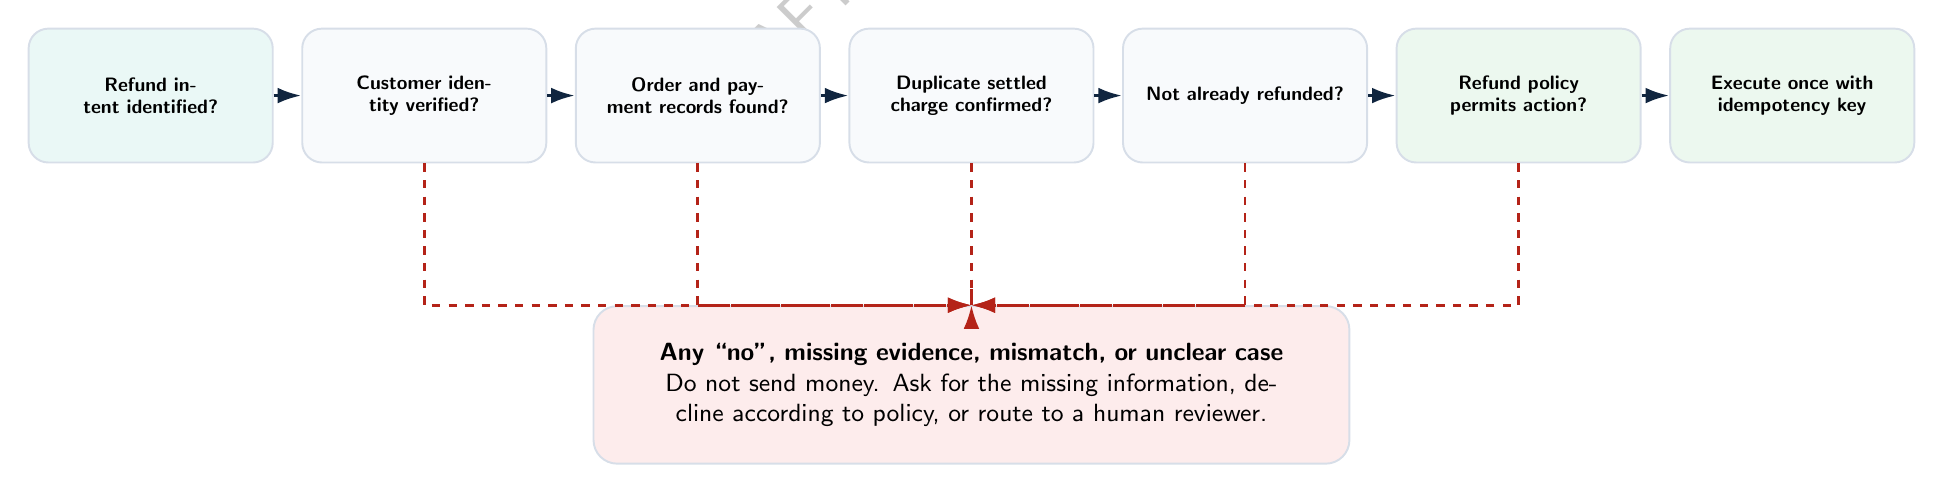
\begin{tikzpicture}[node distance=3.5mm]
  \node[compact,fill=PaleTeal] (intent) {\textbf{Refund intent identified?}};
  \node[compact,fill=Paper,right=of intent] (identity) {\textbf{Customer identity verified?}};
  \node[compact,fill=Paper,right=of identity] (txn) {\textbf{Order and payment records found?}};
  \node[compact,fill=Paper,right=of txn] (dup) {\textbf{Duplicate settled charge confirmed?}};
  \node[compact,fill=Paper,right=of dup] (history) {\textbf{Not already refunded?}};
  \node[compact,fill=PaleGreen,right=of history] (policy) {\textbf{Refund policy permits action?}};
  \node[compact,fill=PaleGreen,right=of policy] (execute) {\textbf{Execute once with idempotency key}};

  \draw[arrow] (intent) -- (identity);
  \draw[arrow] (identity) -- (txn);
  \draw[arrow] (txn) -- (dup);
  \draw[arrow] (dup) -- (history);
  \draw[arrow] (history) -- (policy);
  \draw[arrow] (policy) -- (execute);

  \node[flow,fill=PaleRed,text width=90mm,below=18mm of dup] (review) {\textbf{Any ``no'', missing evidence, mismatch, or unclear case}\\Do not send money. Ask for the missing information, decline according to policy, or route to a human reviewer.};

  \foreach \n in {identity,txn,dup,history,policy}{
    \draw[reviewarrow] (\n.south) |- (review.north);
  }
\end{tikzpicture}
\end{center}

\vspace{4mm}
\begin{minipage}[t]{0.32\textwidth}
\begin{tcolorbox}[border,colback=PaleRed]
\textbf{Confidence is not evidence}\par
A high model probability cannot replace a missing ledger entry, settlement status, or refund record.
\end{tcolorbox}
\end{minipage}\hfill
\begin{minipage}[t]{0.32\textwidth}
\begin{tcolorbox}[border,colback=PaleGreen]
\textbf{Idempotency is mandatory}\par
Use a stable operation key so retries cannot issue the same refund twice.
\end{tcolorbox}
\end{minipage}\hfill
\begin{minipage}[t]{0.32\textwidth}
\begin{tcolorbox}[border,colback=PaleBlue]
\textbf{Explain only after confirmation}\par
The LLM receives the final status and reference from the backend, not a guessed outcome.
\end{tcolorbox}
\end{minipage}

\vspace{3mm}
\begin{tcolorbox}[clean,colback=Navy,coltext=white]
\centering
{\Large\bfseries JEV ROUTES \quad $\cdot$ \quad RULES AUTHORIZE \quad $\cdot$ \quad PAYMENT CONFIRMS}
\end{tcolorbox}

\newpage

% PAGE 5
\pageheading{Implementation snapshot}{KEEP MODEL OUTPUT INSIDE A CONTROLLED WORKFLOW}

\begin{minipage}[t]{0.48\textwidth}
{\large\bfseries\color{Navy} Illustrative focused output}\par
{\scriptsize\color{Muted}Example shape only. This is not a live Jev response.}
\begin{lstlisting}[style=netsetos]
{
  "department": {
    "value": "billing",
    "probability": 0.97
  },
  "urgency": {
    "score": 1.4
  },
  "refund_requested": {
    "value": true,
    "probability": 0.95
  }
}
\end{lstlisting}
\end{minipage}\hfill
\begin{minipage}[t]{0.48\textwidth}
{\large\bfseries\color{Navy} Deterministic authorization logic}\par
{\scriptsize\color{Muted}The application, not the model, owns this gate.}
\begin{lstlisting}[style=netsetos]
if not identity_verified:
    return REVIEW

payment = lookup_order_and_payments()

eligible = (
    payment.duplicate_charge
    and payment.settled
    and not payment.already_refunded
    and policy_allows_refund(payment)
)

if not eligible:
    return REVIEW_OR_DECLINE

return refund_once(
    payment_id=payment.id,
    idempotency_key=case_id
)
\end{lstlisting}
\end{minipage}

\vspace{4mm}
\begin{tcolorbox}[border,colback=PaleBlue]
{\large\bfseries\color{Blue} Confirmed facts $\rightarrow$ LLM $\rightarrow$ customer explanation}\par
\vspace{2mm}
\textbf{Backend facts:} refund status = successful; reference = RF-48219; amount = confirmed amount; expected settlement window = confirmed window.\par
\textbf{Safe response:} ``The duplicate payment has been refunded. Your refund reference is RF-48219. The amount and expected timing shown here come from the confirmed transaction record.''
\end{tcolorbox}

\vspace{3mm}
\begin{minipage}[t]{0.64\textwidth}
\begin{tcolorbox}[border,colback=white]
\textbf{Production evaluation checklist}\par
\pill{PaleTeal}{DECISION ACCURACY}\hspace{2mm}
\pill{PaleTeal}{CALIBRATION}\hspace{2mm}
\pill{PaleBlue}{LATENCY}\hspace{2mm}
\pill{PaleBlue}{COST}\hspace{2mm}
\pill{PaleGreen}{FALSE-ACTION RATE}\hspace{2mm}
\pill{PaleGreen}{ESCALATION QUALITY}
\par\vspace{2mm}
Test with real ticket language, ambiguous cases, missing records, conflicting records, retries, outages, and already-refunded transactions.
\end{tcolorbox}
\end{minipage}\hfill
\begin{minipage}[t]{0.33\textwidth}
\begin{tcolorbox}[border,colback=Paper]
\textbf{Official references}\par
\href{https://docs.typesafe.ai/concepts/system-one}{TypeSafe AI: System One}\par
\href{https://typesafe.ai/blog/introducing-system-one-models-and-jev}{TypeSafe AI: Introducing Jev}\par
\href{https://vercel.com/kb/guide/typesafe-jev-and-ai-sdk}{Vercel: classify, route, and score with Jev}\par
\vspace{1mm}{\scriptsize Checked 20 September 2026. Educational reference; not a TypeSafe publication or a live model test.}
\end{tcolorbox}
\end{minipage}

\vfill
\begin{tcolorbox}[clean,colback=Navy,coltext=white]
\centering
{\Large\bfseries JEV ROUTES \quad $\cdot$ \quad CODE VERIFIES + ACTS \quad $\cdot$ \quad LLM EXPLAINS}
\par\vspace{1mm}{\small Choose every component using measured accuracy, latency, cost, and operational risk.}
\end{tcolorbox}

\end{document}
